\begin{figure}[H]
    \centering
    

\tikzset{every picture/.style={line width=0.75pt}} %set default line width to 0.75pt        

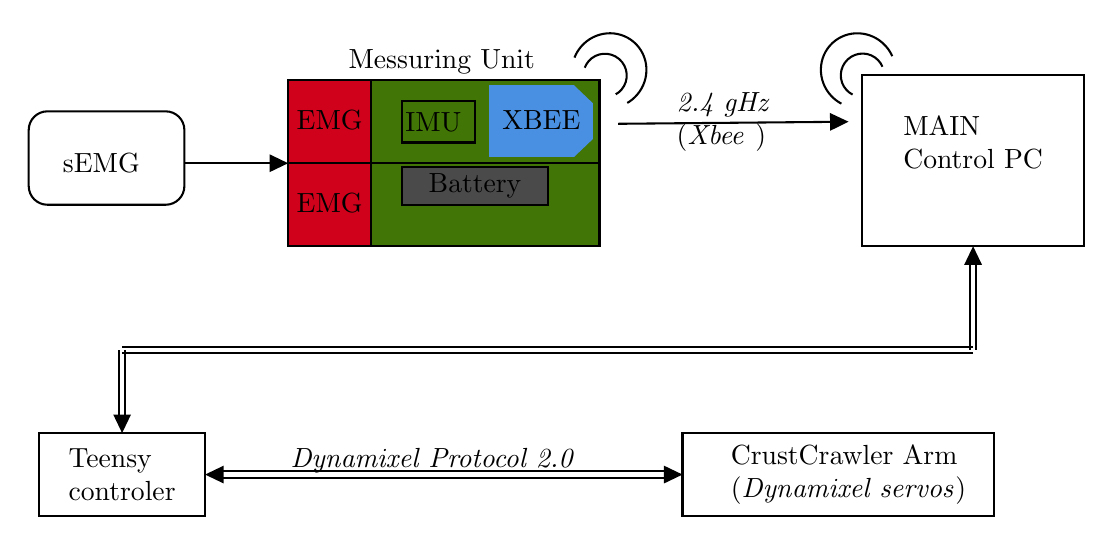
\begin{tikzpicture}[x=0.75pt,y=0.75pt,yscale=-1,xscale=1]
%uncomment if require: \path (0,278.7142848968506); %set diagram left start at 0, and has height of 278.7142848968506

%Shape: Rectangle [id:dp9058146125823148] 
\draw   (436.69,27.6) -- (543.37,27.6) -- (543.37,110) -- (436.69,110) -- cycle ;
%Rounded Rect [id:dp9198394438295476] 
\draw   (35,54) .. controls (35,49.03) and (39.03,45) .. (44,45) -- (101,45) .. controls (105.97,45) and (110,49.03) .. (110,54) -- (110,81) .. controls (110,85.97) and (105.97,90) .. (101,90) -- (44,90) .. controls (39.03,90) and (35,85.97) .. (35,81) -- cycle ;
%Straight Lines [id:da08300314610956905] 
\draw    (110,70) -- (158,70) ;
\draw [shift={(160,70)}, rotate = 180] [fill={rgb, 255:red, 0; green, 0; blue, 0 }  ][line width=0.75]  [draw opacity=0] (8.93,-4.29) -- (0,0) -- (8.93,4.29) -- cycle    ;

%Shape: Rectangle [id:dp49994760485296896] 
\draw  [fill={rgb, 255:red, 65; green, 117; blue, 5 }  ,fill opacity=1 ] (160,30) -- (310,30) -- (310,110) -- (160,110) -- cycle ;
%Shape: Rectangle [id:dp9990642544965083] 
\draw  [fill={rgb, 255:red, 208; green, 2; blue, 27 }  ,fill opacity=1 ] (160,30) -- (200,30) -- (200,70) -- (160,70) -- cycle ;
%Shape: Rectangle [id:dp5155575250253981] 
\draw  [fill={rgb, 255:red, 208; green, 2; blue, 27 }  ,fill opacity=1 ] (160,70) -- (200,70) -- (200,110) -- (160,110) -- cycle ;
%Straight Lines [id:da2266079205645528] 
\draw    (319,51) -- (428,50.02) ;
\draw [shift={(430,50)}, rotate = 539.48] [fill={rgb, 255:red, 0; green, 0; blue, 0 }  ][line width=0.75]  [draw opacity=0] (8.93,-4.29) -- (0,0) -- (8.93,4.29) -- cycle    ;

%Shape: Rectangle [id:dp7097032559017205] 
\draw  [fill={rgb, 255:red, 65; green, 117; blue, 5 }  ,fill opacity=1 ] (200,30) -- (310,30) -- (310,70) -- (200,70) -- cycle ;
%Shape: Rectangle [id:dp16739603109917534] 
\draw  [fill={rgb, 255:red, 65; green, 117; blue, 5 }  ,fill opacity=1 ] (200,70) -- (310,70) -- (310,110) -- (200,110) -- cycle ;
%Shape: Diagonal Stripe [id:dp825501516378429] 
\draw  [color={rgb, 255:red, 0; green, 0; blue, 0 }  ,draw opacity=0 ][fill={rgb, 255:red, 74; green, 144; blue, 226 }  ,fill opacity=1 ] (306.79,58.36) -- (297.73,67) -- (297.73,32.43) -- (306.79,41.07) -- cycle ;
%Shape: Rectangle [id:dp443446878421101] 
\draw  [draw opacity=0][fill={rgb, 255:red, 74; green, 144; blue, 226 }  ,fill opacity=1 ] (257,32.43) -- (297.73,32.43) -- (297.73,67) -- (257,67) -- cycle ;

%Shape: Rectangle [id:dp7890442898232035] 
\draw  [fill={rgb, 255:red, 74; green, 74; blue, 74 }  ,fill opacity=1 ] (215,72) -- (285,72) -- (285,90) -- (215,90) -- cycle ;
%Shape: Rectangle [id:dp3185767197775584] 
\draw  [fill={rgb, 255:red, 65; green, 117; blue, 5 }  ,fill opacity=1 ] (215,40) -- (250,40) -- (250,60) -- (215,60) -- cycle ;
%Shape: Arc [id:dp6014275798651711] 
\draw  [draw opacity=0] (302.89,23.99) .. controls (303.31,22.88) and (303.92,21.82) .. (304.74,20.86) .. controls (308.48,16.5) and (315.08,16.02) .. (319.46,19.79) .. controls (323.85,23.55) and (324.37,30.14) .. (320.63,34.5) .. controls (319.81,35.46) and (318.86,36.23) .. (317.82,36.8) -- (312.69,27.68) -- cycle ; \draw   (302.89,23.99) .. controls (303.31,22.88) and (303.92,21.82) .. (304.74,20.86) .. controls (308.48,16.5) and (315.08,16.02) .. (319.46,19.79) .. controls (323.85,23.55) and (324.37,30.14) .. (320.63,34.5) .. controls (319.81,35.46) and (318.86,36.23) .. (317.82,36.8) ;
%Shape: Arc [id:dp584505117797834] 
\draw  [draw opacity=0] (297.95,19.11) .. controls (298.69,17.23) and (299.75,15.44) .. (301.14,13.82) .. controls (307.69,6.19) and (319.05,5.19) .. (326.5,11.59) .. controls (333.96,17.98) and (334.69,29.36) .. (328.14,36.99) .. controls (326.75,38.61) and (325.14,39.94) .. (323.39,40.95) -- (314.64,25.4) -- cycle ; \draw   (297.95,19.11) .. controls (298.69,17.23) and (299.75,15.44) .. (301.14,13.82) .. controls (307.69,6.19) and (319.05,5.19) .. (326.5,11.59) .. controls (333.96,17.98) and (334.69,29.36) .. (328.14,36.99) .. controls (326.75,38.61) and (325.14,39.94) .. (323.39,40.95) ;

%Shape: Arc [id:dp9643215893864674] 
\draw  [draw opacity=0] (431.94,36.92) .. controls (430.88,36.39) and (429.9,35.66) .. (429.04,34.74) .. controls (425.12,30.54) and (425.37,23.93) .. (429.6,19.99) .. controls (433.82,16.04) and (440.43,16.25) .. (444.35,20.46) .. controls (445.21,21.38) and (445.87,22.41) .. (446.33,23.51) -- (436.69,27.6) -- cycle ; \draw   (431.94,36.92) .. controls (430.88,36.39) and (429.9,35.66) .. (429.04,34.74) .. controls (425.12,30.54) and (425.37,23.93) .. (429.6,19.99) .. controls (433.82,16.04) and (440.43,16.25) .. (444.35,20.46) .. controls (445.21,21.38) and (445.87,22.41) .. (446.33,23.51) ;
%Shape: Arc [id:dp6589182805450249] 
\draw  [draw opacity=0] (426.55,41.3) .. controls (424.76,40.36) and (423.1,39.1) .. (421.64,37.54) .. controls (414.78,30.18) and (415.04,18.79) .. (422.22,12.09) .. controls (429.41,5.39) and (440.79,5.91) .. (447.65,13.27) .. controls (449.11,14.83) and (450.25,16.58) .. (451.07,18.43) -- (434.64,25.4) -- cycle ; \draw   (426.55,41.3) .. controls (424.76,40.36) and (423.1,39.1) .. (421.64,37.54) .. controls (414.78,30.18) and (415.04,18.79) .. (422.22,12.09) .. controls (429.41,5.39) and (440.79,5.91) .. (447.65,13.27) .. controls (449.11,14.83) and (450.25,16.58) .. (451.07,18.43) ;

%Straight Lines [id:da8446148813559833] 
\draw    (491.5,118) -- (491.5,160)(488.5,118) -- (488.5,160) ;

\draw [shift={(490,110)}, rotate = 90] [fill={rgb, 255:red, 0; green, 0; blue, 0 }  ][line width=0.75]  [draw opacity=0] (8.93,-4.29) -- (0,0) -- (8.93,4.29) -- cycle    ;
%Straight Lines [id:da5044267925519024] 
\draw    (490,161.5) -- (80,161.5)(490,158.5) -- (80,158.5) ;


%Straight Lines [id:da7406026285596496] 
\draw    (81.5,160) -- (81.5,192)(78.5,160) -- (78.5,192) ;
\draw [shift={(80,200)}, rotate = 270] [fill={rgb, 255:red, 0; green, 0; blue, 0 }  ][line width=0.75]  [draw opacity=0] (8.93,-4.29) -- (0,0) -- (8.93,4.29) -- cycle    ;

%Shape: Rectangle [id:dp016623272212034745] 
\draw   (40,200) -- (120,200) -- (120,240) -- (40,240) -- cycle ;
%Straight Lines [id:da7263406511929] 
\draw    (128,218.5) -- (342,218.5)(128,221.5) -- (342,221.5) ;
\draw [shift={(350,220)}, rotate = 180] [fill={rgb, 255:red, 0; green, 0; blue, 0 }  ][line width=0.75]  [draw opacity=0] (8.93,-4.29) -- (0,0) -- (8.93,4.29) -- cycle    ;
\draw [shift={(120,220)}, rotate = 0] [fill={rgb, 255:red, 0; green, 0; blue, 0 }  ][line width=0.75]  [draw opacity=0] (8.93,-4.29) -- (0,0) -- (8.93,4.29) -- cycle    ;
%Shape: Rectangle [id:dp6457555540924869] 
\draw   (350,200) -- (500,200) -- (500,240) -- (350,240) -- cycle ;

% Text Node
\draw (490,60) node  [align=left] {MAIN\\Control PC};
% Text Node
\draw (70,70) node  [align=left] {sEMG};
% Text Node
\draw (234,21) node  [align=left] {Messuring Unit};
% Text Node
\draw (282,49) node  [align=left] {XBEE};
% Text Node
\draw (370,50) node  [align=left] {\textit{2.4 gHz}\\(\textit{Xbee })};
% Text Node
\draw (250,81) node  [align=left] {Battery};
% Text Node
\draw (180,49) node  [align=left] {EMG};
% Text Node
\draw (180,89) node  [align=left] {EMG};
% Text Node
\draw (230,50) node  [align=left] {IMU};
% Text Node
\draw (80,220) node  [align=left] {Teensy\\controler};
% Text Node
\draw (230,220) node  [align=left] {\textit{Dynamixel Protocol 2.0}\\};
% Text Node
\draw (430,220) node  [align=left] {CrustCrawler Arm\\(\textit{Dynamixel servos})};


\end{tikzpicture}

    \caption{Data flowchart}
    \label{fig:DataFlow}
\end{figure}